
In order to solve the optimal control problem \eqref{AdvDiff}, or \eqref{AdvDiff_Linear}, some inputs must be provided. The desired state $\widehat \rho$, the PDE source term $f$, and the external potential $V_{ext}$ must be given. Furthermore, an initial condition for $\rho$, the final time condition for $\adj$ and an initial guess for the control $\vec{w}$ have to be be specified. 
The interaction kernel (++ terminology? ++) is of the form:
\begin{align*}
\vec{K} = \nabla V_2, \qquad V_2 = e^{-x^2}.
\end{align*}
Three interaction strengths are considered. Firstly, the problem is solved without an interaction term present ($\gamma = 0$). Then the considered problem is solved with an order one attractive interaction term ($\gamma = -1$) and an order one repulsive interaction term ($\gamma = 1$), respectively. Initially, the control $\vec{w}$ is set to zero. It is then investigated how the control changes from this baseline, influenced by the different interaction strengths. This is considered for different values of the regularization parameter $\beta$ and it is expected that the control will increase with decreasing $\beta$, since the cost functional in problems \eqref{AdvDiff} and \eqref{AdvDiff_Linear} allows for a larger control with smaller $\beta$.
In the following examples, the domain considered is $\Omega \times [0,T] = [-1,1] \times [0,1]$. The number of spatial points is $N=40$, and the number of time points is $n=41$ (++will be changed++). The tolerances in the ODE solver are set to $10^{-8}$ and the tolerance for the convergence of the optimization algorithm is $10^{-4}$. The mixing parameter $\lambda$ is $0.01$, unless stated otherwise.
\subsection{Nonlinear control problems with an additional nonlocal integral term 1D} \label{sec:Examples1d}
Examples of solving Problem \eqref{AdvDiff}, with 'no-flux type' boundary conditions \eqref{NoFlux} and Dirichlet boundary conditions \eqref{Dirichlet} are given in this section. 
 
\subsubsection{Neumann boundary conditions, Example 1}	 
The chosen inputs for this example are:
\begin{align*}
\widehat \rho &= \frac{1}{2}(1-t) + t\bigg(\frac{1}{2}\sin(\pi (y - 2)/2) + \frac{1}{2}\bigg)\\
\rho_{0} &= \frac{1}{2}\\
\adj_{T} &= 0\\
\vec{w} &= 0\\
f &=0\\
V_{ext} &=0
\end{align*}	
Table \ref{TabNFlowEx1} displays the results for this example. The value of the cost functional for the uncontrolled case ($J_{uc}$) is compared with the controlled case ($J_{c}$) for different values of $\beta$ and for each of the interaction strengths. It can be observed that in all cases $J_{c}$ will be lower or equal value to $J_{uc}$. The lowest values of $J_{c}$ will be observed for the smallest $\beta$ value considered. At large values of $\beta$, applying control is heavily penalised and the optimal control approaches zero, which coincides with the uncontrolled case. Furthermore, Table \ref{TabNFlowEx1} displays the number of iterations for each of these examples. The desired state $\widehat \rho$, and $\rho_{uc}$ for $\gamma =1$ and $\gamma = -1$, with $\beta =10^{-3}$ are shown in Figure \ref{Ex12DN1}. The desired state $\hat \rho$ and $\rho_{uc}$ are independent of $\beta$. However, $\rho_{uc}$ changes considerably with the choice of interaction strength $\gamma$. The optimal states $\rho$ for $\gamma = 1,0,-1$ and corresponding optimal controls, with $\beta = 10^{-3}$ are shown in Figure \ref{Ex12DN2}. 
It can be observed that in the case of $\beta = 10^{-3}$, the optimal state $\rho$ is very similar to $\hat \rho$, regardless of the choice of interaction. For larger values of $\beta$, the optimal $\rho$ displays qualitative differences, depending on the interaction term. 
\begin{figure}[h]
	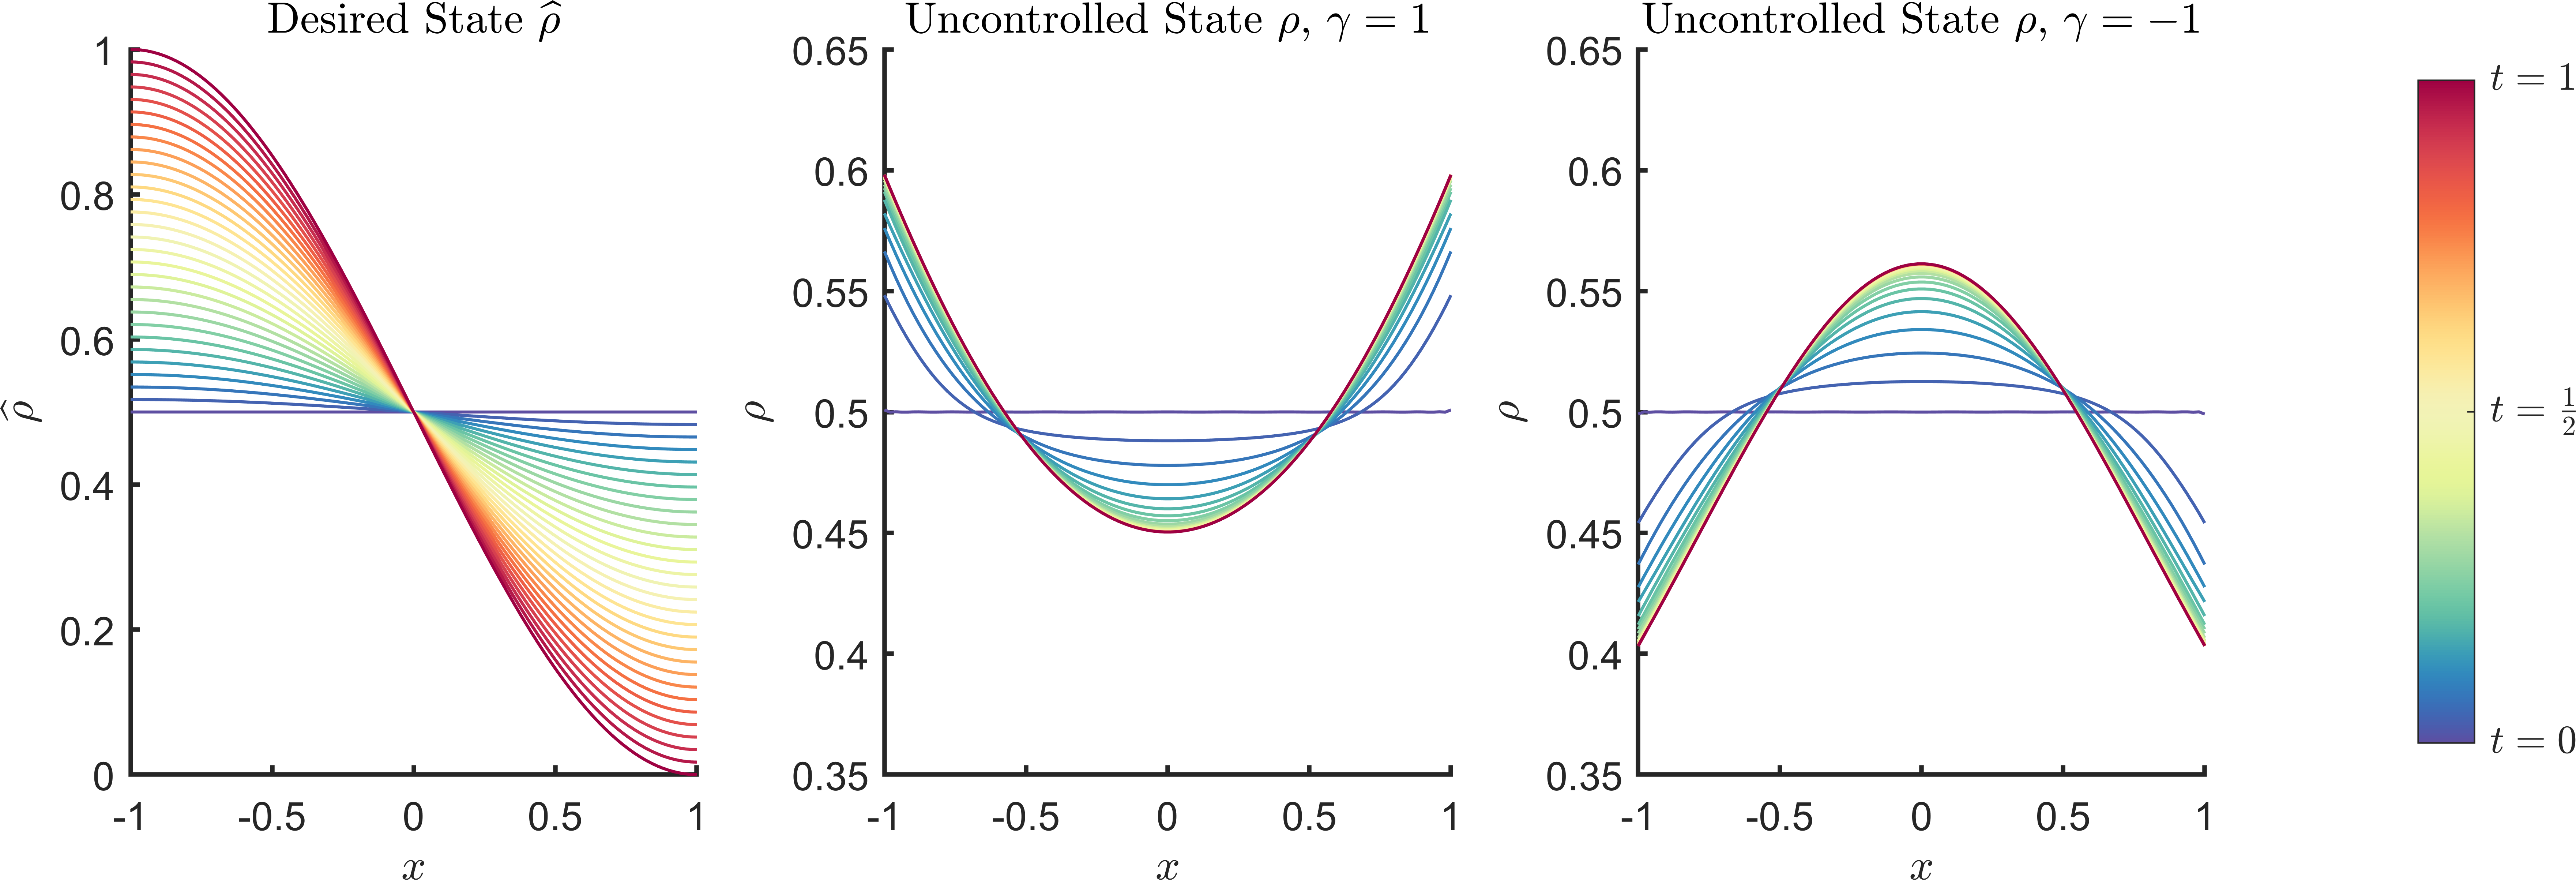
\includegraphics[scale=0.25]{Figure1.png}
	\caption{Example 1, desired state $\widehat \rho$ and $\rho_{uc}$ at $\gamma =1$ and $\gamma =-1$, $\beta = 10^{-3}$}
	\label{Ex12DN1}
\end{figure}
\begin{figure}[h]
	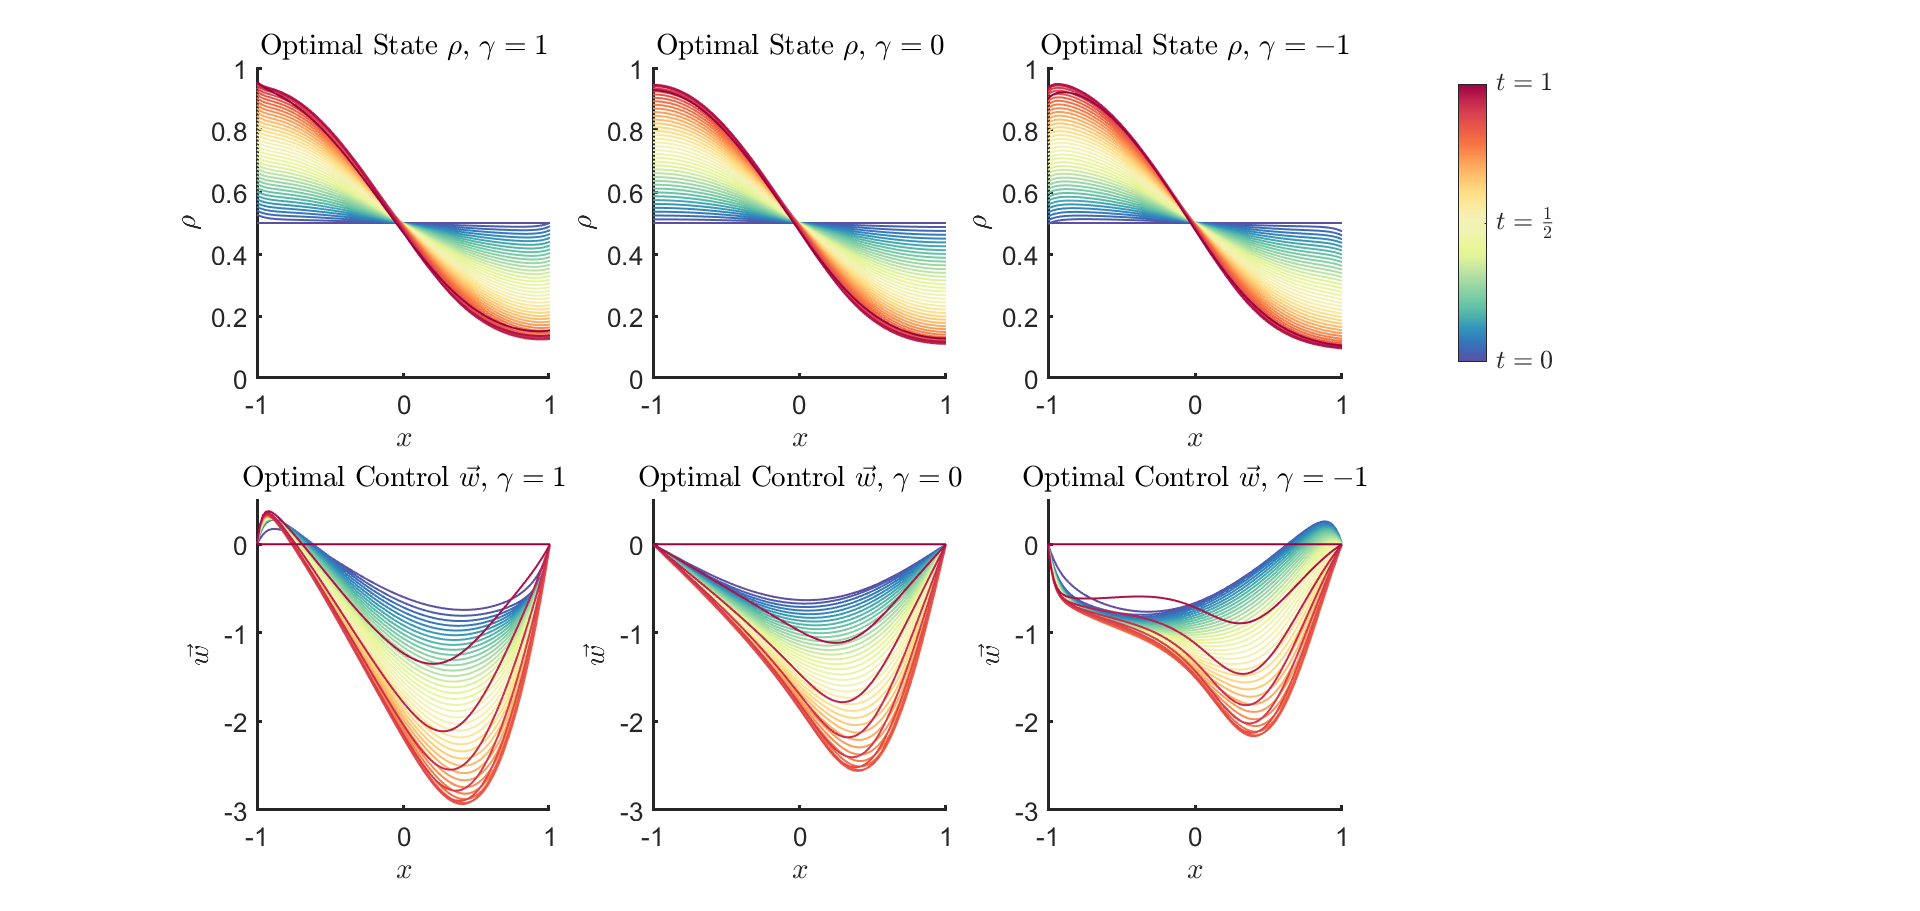
\includegraphics[scale=0.25]{Figure2.png}
	\caption{Example 1, optimal solutions $\rho$ for $\gamma = 1,0,-1$ and corresponding optimal controls $\vec{w}$, $\beta = 10^{-3}$.}
	\label{Ex12DN2}
\end{figure}


\begin{table}[h]
	\begin{tabular}{ ||c|| c | c |c | c ||}
		\hline
		$\beta$ / $\gamma$ & $10^{-3}$  & $10^{-1}$  & $10$ & $10^3$ \\ 
		\hline 
		      & $J_{uc} = 0.0438$ & $J_{uc} = 0.0438$  & $J_{uc} = 0.0438$ & $J_{uc} = 0.0438$\\ 
		 $-1$ & $J_c = 0.0011$ & $J_c = 0.0270$ & $J_c = 0.0435$ & $J_c = 0.0438$\\ 
		      & Iter. $= 667$ & Iter. $= 649$  & Iter. $= 468$ & Iter. $= 13$\\ 
		 \hline
		      & $J_{uc} = 0.0417$ & $J_{uc} = 0.0417$   & $J_{uc} = 0.0417$& $J_{uc} = 0.0417$\\
		 $0$  & $J_c = 0.0014$ & $J_c = 0.0283$  & $J_c = 0.0415$ & $J_c = 0.0417$\\ 
		      & Iter. $= 671$ & Iter. $= 656$  & Iter. $= 434$ & Iter. $= 1$\\ 
		 \hline
		      & $J_{uc} = 0.0434$ & $J_{uc} = 0.0434$  & $J_{uc} = 0.0434$ & $J_{uc} = 0.0434$\\
		 $1$  & $J_c = 0.0020$ & $J_c = 0.0324$  & $J_c = 0.0432$ & $J_c = 0.0434$\\ 
		      & Iter. $= 674$ & Iter. $= 686$  & Iter. $= 411$ & Iter. $= 1$\\ 
		 \hline 
	\end{tabular}
    \caption{}
    \label{TabNFlowEx1}
\end{table}

\subsubsection{Neumann boundary conditions, Example 2} 
The chosen inputs for Example 2 are:
\begin{align*}
\widehat \rho &= \bigg(\frac{1}{2}\cos(\pi y) + \frac{1}{2}\bigg)(1-t) + t\bigg(-\frac{1}{2}\cos(2 \pi y) + \frac{1}{2}\bigg)\\
\rho_{0} &= \frac{1}{2}\cos(\pi y) + \frac{1}{2}\\
\adj_{T} &= 0\\
\vec{w} &= 0\\
f &=0\\
V_{ext} &=0
\end{align*}
In Table \ref{TabNFlowEx2} the results for Example 2 are displayed. These are mostly comparable with the results for Example 1. In all three configurations of the interaction term, the control is focussed on transporting the mass from the middle onto two piles centred at $x=-0.5$ and $x=0.5$. In Figure \ref{Ex22DN1}, the desired state $\widehat \rho$, the optimal state $\rho$ and the optimal control $\vec{w}$ are displayed for $\beta = 10^{-3}$, and compared to Example 3 below. 
\begin{figure}[h]
	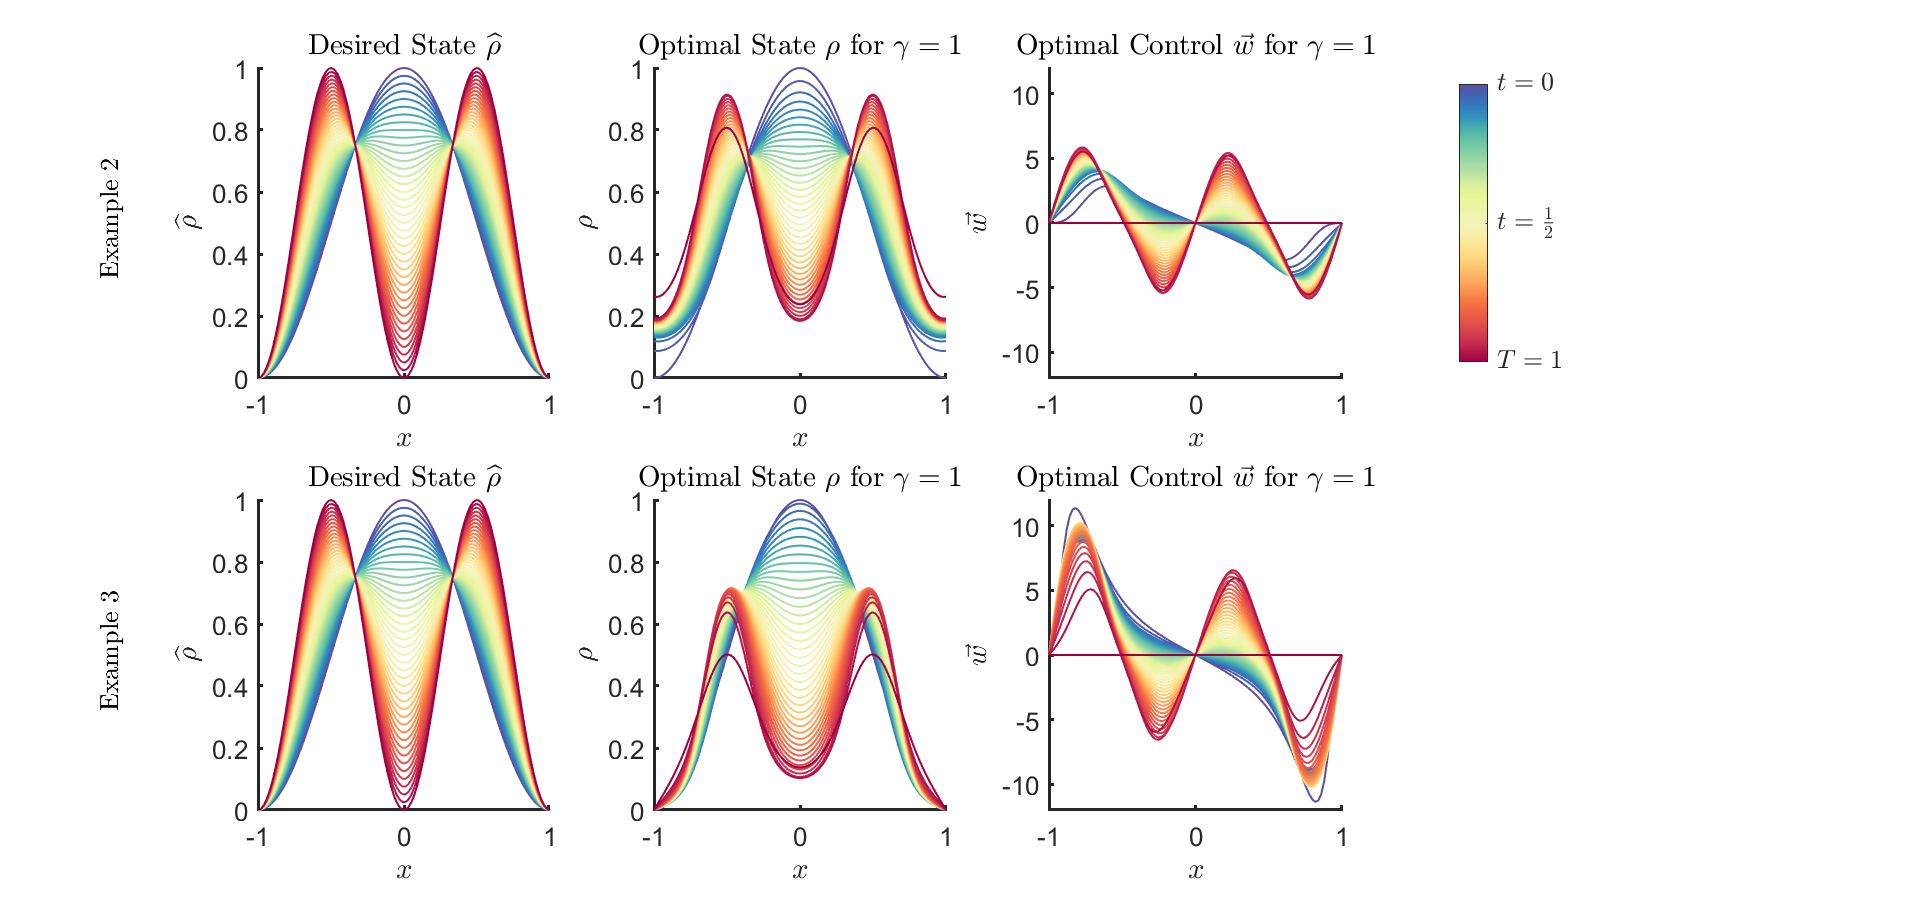
\includegraphics[scale=0.25]{Figure3.png}
	\caption{Example 2/ Example 3, desired state $\widehat \rho$, optimal state $\rho$ and corresponding optimal control $\vec{w}$, $\beta = 10^{-3}$, $\gamma = 1$.}
	\label{Ex22DN1}
\end{figure}

\begin{table}
	\begin{tabular}{ ||c|| c | c |c | c ||}
		\hline
		$\beta$ / $\gamma$ & $10^{-3}$  & $10^{-1}$  & $10$ & $10^3$ \\ 
		\hline 
		& $J_{uc} = 0.0536$ & $J_{uc} = 0.0536$  & $J_{uc} = 0.0536$ & $J_{uc} = 0.0536$\\ 
		$-1$ & $J_c = 0.0096$ & $J_c = 0.0493$ & $J_c = 0.0535$ & $J_c = 0.0536$\\ 
		& Iter. $= 724$ & Iter. $= 769$  & Iter. $= 379$ & Iter. $= 1$\\ 
		\hline
		& $J_{uc} = 0.0669$ & $J_{uc} = 0.0669$   & $J_{uc} = 0.0669$& $J_{uc} = 0.0669$\\
		$0$  & $J_c = 0.0109$ & $J_c = 0.0603$  & $J_c = 0.0668$ & $J_c = 0.0669$\\ 
		& Iter. $= 726$ & Iter. $= 770$  & Iter. $= 390$ & Iter. $= 1$\\ 
		\hline
		& $J_{uc} = 0.0839$ & $J_{uc} = 0.0839$  & $J_{uc} = 0.0839$ & $J_{uc} = 0.0839$\\
		$1$  & $J_c = 0.0125$ & $J_c = 0.0749$  & $J_c = 0.0838$ & $J_c = 0.0839$\\ 
		& Iter. $= 728$ & Iter. $= 772$  & Iter. $= 396$ & Iter. $= 1$\\ 
		\hline 
	\end{tabular}
    \caption{}
    \label{TabNFlowEx2}
\end{table}

\subsubsection{Dirichlet boundary conditions, Example 3} 
The inputs for this example are:
\begin{align*}
\widehat \rho &= \bigg(\frac{1}{2}\cos(\pi y) + \frac{1}{2}\bigg)(1-t) + t\bigg(-\frac{1}{2}\cos(2 \pi y) + \frac{1}{2}\bigg)\\
\rho_{0} &= \frac{1}{2}\cos(\pi y) + \frac{1}{2}\\
\adj_{T} &= 0\\
\vec{w} &= 0\\
f &=0\\
V_{ext} &=0
\end{align*}
Table \ref{TabNFlowEx3} presents the results for this example for a range of $\beta$ values and different interaction strengths. The observations are in line with those in Example 1 and 2. In particular, $ \widehat \rho$ and $\rho_0$ coincide with those of the Neumann problem in Example 2. The comparison between results can be seen in Figure \ref{Ex22DN1}. Both the optimal state $\rho$ and the optimal control are qualitatively different when considering Dirichlet boundary conditions over Neumann conditions.

\begin{table}
	\begin{tabular}{ ||c|| c | c |c | c ||}
		\hline
		$\beta$ / $\gamma$ & $10^{-3}$  & $10^{-1}$  & $10$ & $10^3$ \\ 
		\hline 
		& $J_{uc} = 0.0510$ & $J_{uc} = 0.0510$  & $J_{uc} = 0.0510$ & $J_{uc} = 0.0510$\\ 
		$-1$ & $J_c = 0.0026$ & $J_c = 0.0365$ & $J_c = 0.0508$ & $J_c = 0.0510$\\ 
		& Iter. $= 690$ & Iter. $= 696$  & Iter. $= 696$ & Iter. $= 696$\\ 
		\hline
		& $J_{uc} = 0.0417$ & $J_{uc} = 0.0417$  & $J_{uc} = 0.0417$& $J_{uc} = 0.0417$\\
		$0$  & $J_c = 0.0027$ & $J_c = 0.0343$  & $J_c = 0.0416$ & $J_c = 0.0417$\\ 
		& Iter. $= 696$ & Iter. $= 742$  & Iter. $= 409$ & Iter. $= 1$\\ 
		\hline
		& $J_{uc} = 0.0452$ & $J_{uc} = 0.0452$  & $J_{uc} = 0.0452$ & $J_{uc} = 0.0452$\\
		$1$  & $J_c = 0.0030$ & $J_c = 0.0388$  & $J_c = 0.0452$ & $J_c = 0.0452$\\ 
		& Iter. $= 703$ & Iter. $= 779$  & Iter. $= 397$ & Iter. $= 1$\\ 
		\hline 
	\end{tabular}
	\caption{Update table! Is for different example}
	\label{TabNFlowEx3}
\end{table}


\subsection{Linear control problems with an additional nonlocal integral term}
In this section, examples of solving Problem \eqref{AdvDiff_Linear} with both 'no-flux type' boundary conditions \eqref{NoFlux_Linear} and Dirichlet boundary conditions \eqref{Dirichlet}.
\subsubsection{Dirichlet boundary conditions, Example 4}
++ If kept maybe change $\widehat \rho$ and $\rho_0$? Same as Examples 2 and 3 / or compare to 2 and 3? ++
The inputs for this example are:
\begin{align*}
\widehat \rho &= (1 - t)\bigg(\frac{1}{2}\cos(\pi y) + \frac{1}{2}\bigg)  + t\bigg(-\frac{1}{2}\cos(\pi y) + \frac{1}{2}\bigg)\\
\rho_{0} &= \frac{1}{2}\cos(\pi y) + \frac{1}{2}\\
\adj_{T} &= 0\\
{w} &= 0\\
f &=0\\
V_{ext} &=0
\end{align*}
In Table \ref{TabNFlowEx4} the results for Example 4 for a range of parameter values can be found. The results are qualitatively similar to the previous examples, the only difference is that the control is applied linearly in this example.

\begin{table}[h]
	\begin{tabular}{ ||c|| c | c |c | c ||}
		\hline
		$\beta$ / $\gamma$ & $10^{-3}$  & $10^{-1}$  & $10$ & $10^3$ \\ 
		\hline 
		& $J_{uc} = 0.1417$ & $J_{uc} = 0.1417$  & $J_{uc} = 0.1417$ & $J_{uc} = 0.1417$\\ 
		$-1$ & $J_c = 0.0203$ & $J_c = 0.0903$ & $J_c = 0.1407$ & $J_c = 0.1417$\\ 
		& Iter. $= 787$ & Iter. $= 740$  & Iter. $= 503$ & Iter. $= 49$\\ 
		\hline
		& $J_{uc} = 0.1545$ & $J_{uc} = 0.1545$   & $J_{uc} = 0.1545$& $J_{uc} = 0.1545$\\
		$0$  & $J_c = 0.0200$ & $J_c = 0.1015$  & $J_c = 0.1536$ & $J_c = 0.1545$\\ 
		& Iter. $= 791$ & Iter. $= 740$  & Iter. $= 510$ & Iter. $= 56$\\ 
		\hline
		& $J_{uc} = 0.1661$ & $J_{uc} = 0.1661$  & $J_{uc} = 0.1661$ & $J_{uc} = 0.1661$\\
		$1$  & $J_c = 0.0204$ & $J_c = 0.1135$  & $J_c = 0.1652$ & $J_c = 0.1661$\\ 
		& Iter. $= 795$ & Iter. $= 741$  & Iter. $= 515$ & Iter. $= 61$\\ 
		\hline 
	\end{tabular}
	\caption{}
	\label{TabNFlowEx4}
\end{table}


\subsubsection{Neumann boundary conditions, Example 5}
The inputs for this example are:
\begin{align*}
\widehat \rho &= \frac{1}{2}(1-t) + t\frac{1}{2}(-\cos(\pi y) + 1)\\
\rho_{0} &= \frac{1}{2}\\
\adj_{T} &= 0\\
{w} &= 0\\
f &=0\\
V_{ext} &=0
\end{align*}
Table \ref{TabNFlowEx5} shows the results for Example 5. Note that for this example, when $\beta = 10^{-3}$, the mixing parameter $\lambda$ had to be set to $0.001$ (why? explanation needed?).
Again, the only qualitative difference to interpreting the results is that the control is applied linearly.
\begin{table}[h]
	\begin{tabular}{ ||c|| c | c |c | c ||}
		\hline
		$\beta$ / $\gamma$ & $10^{-3}$  & $10^{-1}$  & $10$ & $10^3$ \\ 
		\hline 
		& $J_{uc} = 0.0606$ & $J_{uc} = 0.0606$  & $J_{uc} = 0.0606$ & $J_{uc} = 0.0606$\\ 
		$-1$ & $J_c = 0.0060$ & $J_c = 0.0554$ & $J_c = 0.0606$ & $J_c = 0.0606$\\ 
		& Iter. $= 7311$ & Iter. $= 771$  & Iter. $= 389$ & Iter. $= 1$\\ 
		\hline
		& $J_{uc} = 0.0417$ & $J_{uc} = 0.0417$   & $J_{uc} = 0.0417$& $J_{uc} = 0.0417$\\
		$0$  & $J_c = 0.0045$ & $J_c = 0.0383$  & $J_c = 0.0416$ & $J_c = 0.0417$\\ 
		& Iter. $= 7227$ & Iter. $= 759$  & Iter. $= 364$ & Iter. $= 1$\\ 
		\hline
		& $J_{uc} = 0.0286$ & $J_{uc} = 0.0286$  & $J_{uc} = 0.0286$ & $J_{uc} = 0.0286$\\
		$1$  & $J_c = 0.0036$ & $J_c = 0.0265$  & $J_c = 0.0285$ & $J_c = 0.0286$\\ 
		& Iter. $= 7205$ & Iter. $= 746$  & Iter. $= 341$ & Iter. $= 1$\\ 
		\hline 
	\end{tabular}
	\caption{}
	\label{TabNFlowEx5}
\end{table}


\subsection{Nonlinear control problems with an additional nonlocal integral term 1D}

\subsubsection{Neumann boundary conditions, Example 1}	
We have the following set up:
\begin{align*}
\widehat \rho &= \frac{1}{4}(1-t) + t\bigg(\frac{1}{4}\sin \bigg(\frac{\pi}{2}(x_1 - 2)\bigg)\sin \bigg(\frac{\pi}{2}(x_2 - 2)\bigg) + \frac{1}{4}\bigg)\\
\rho_0 &= \frac{1}{4}\\
q_{T} &= 0\\
\vec{w} &= 0\\
f &=0\\
V_{ext} &=0
\end{align*}
In figures \ref{rhoHat2dEx2} and \ref{rhoOpt2dEx2} the results for this example are illustrated for one choice of parameters. This example is directly comparable to Example 1 in Section \ref{sec:Examples1d}.
\begin{figure}[h]
	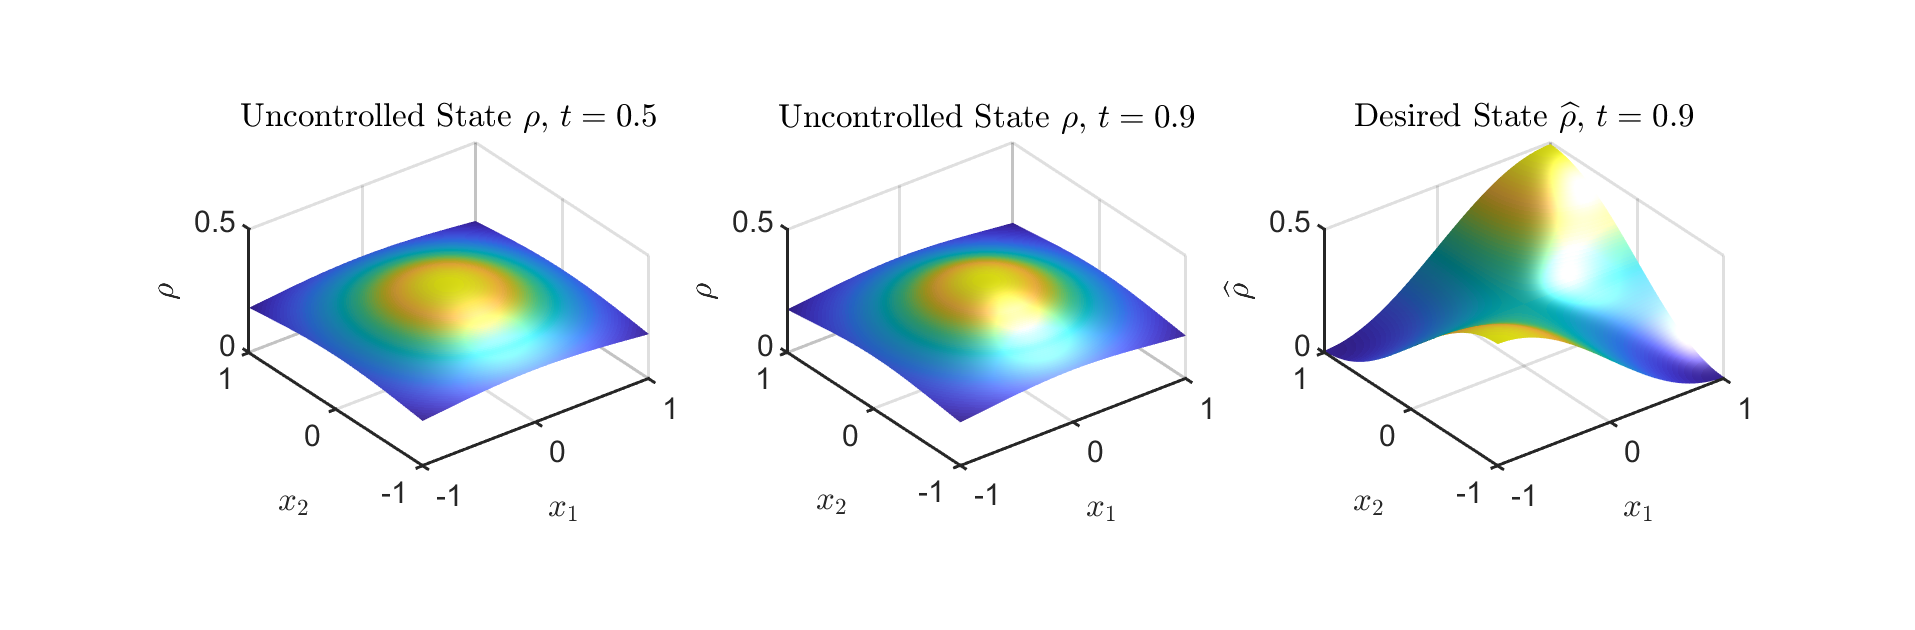
\includegraphics[scale=0.3]{Res1Ex2.png}
	\caption{2D Example 2, uncontrolled $\rho$ and $\widehat \rho$, $\beta = 10^{-3}$, $\gamma = -1$.++Needs update++}
	\label{rhoHat2dEx2}
\end{figure}
\begin{figure}[h]
	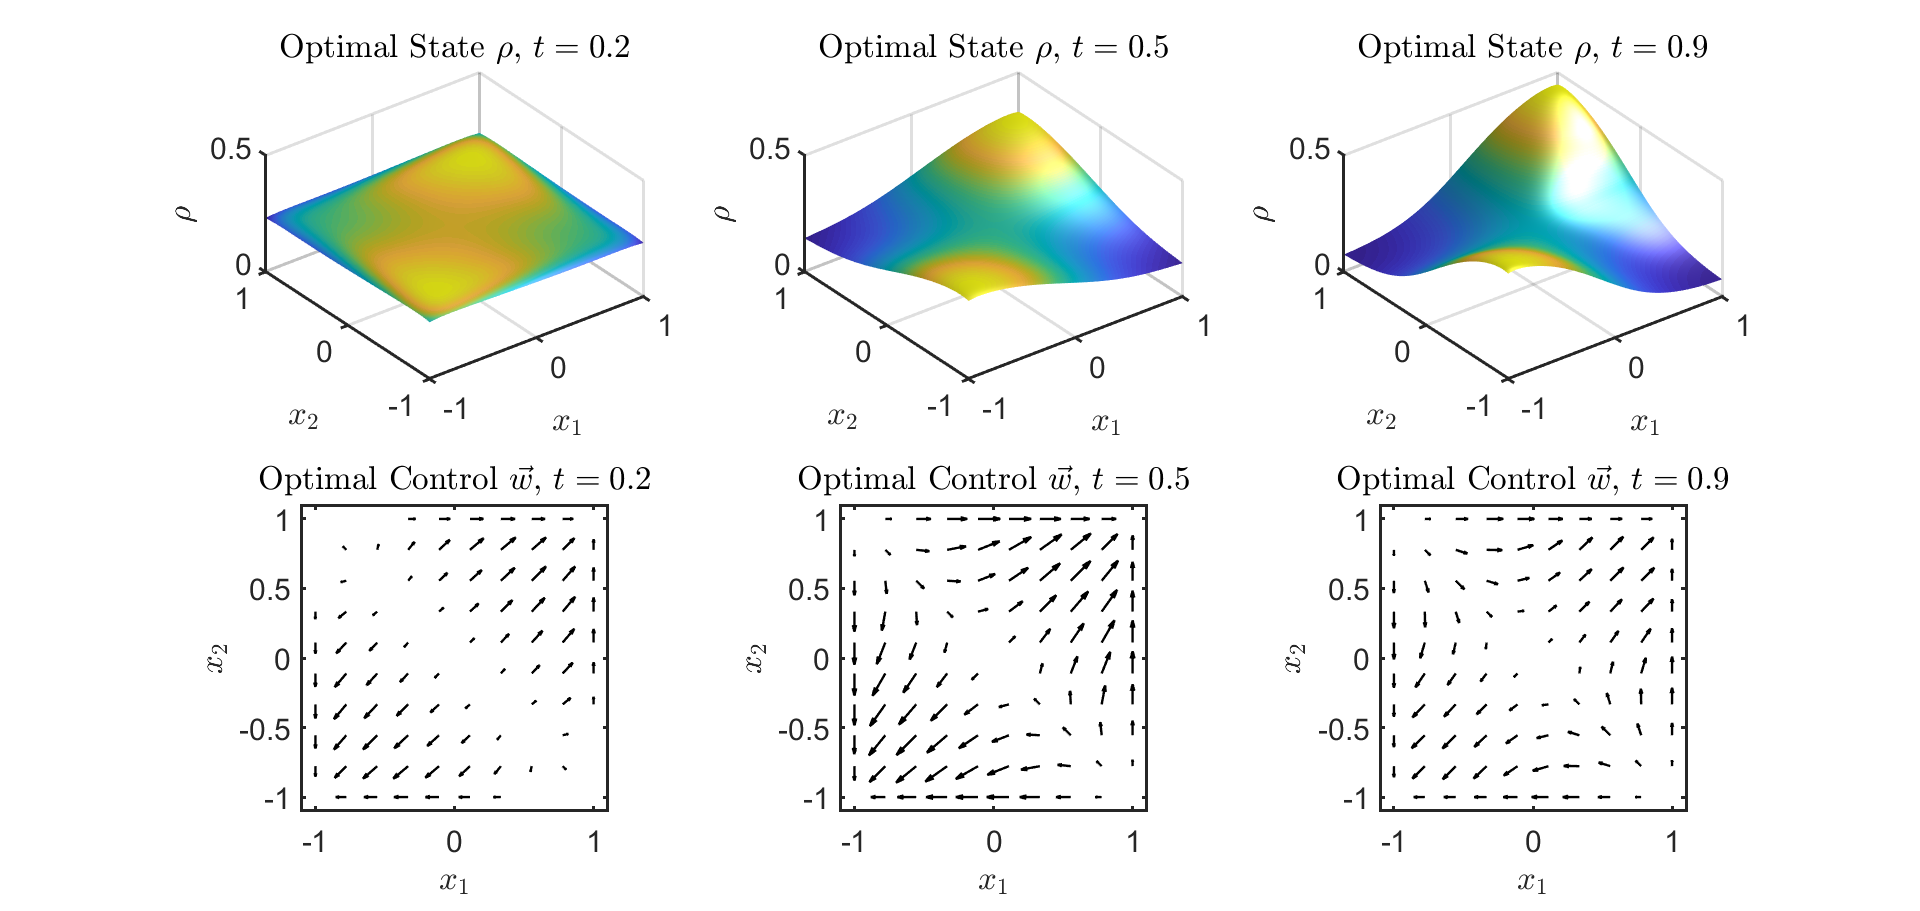
\includegraphics[scale=0.3]{Res2Ex2.png}
	\caption{2D Example 2, controlled $\rho$ and optimal control $\vec{w}$, $\beta = 10^{-3}$, $\gamma = -1$.++Needs update++}
	\label{rhoOpt2dEx2}
\end{figure}


\subsubsection{Neumann boundary conditions, Example 2}	
Here, we have:
\begin{align*}
\widehat \rho &= \frac{1}{4}(1-t) + t\frac{1}{0.9921}e^{-3((y_1+0.2)^2 + (y_2+0.2)^2))}\\
\rho_0 &= \frac{1}{4}\\
q_{T} &= 0\\
\vec{w} &= 0\\
f &=0\\
V_{ext} &=0
\end{align*}
In figures \ref{rhoHat2dEx4} and \ref{rhoOpt2dEx4} the results are illustrated. It can be observed very clearly that the control is driving to the desired state. It is noticeable that the peak of the desired state does not have to be supported as much as the slopes. This is due to the attractive interactions of the particles in this configuration and cannot be observed for repulsive particles.

\begin{figure}[h]
	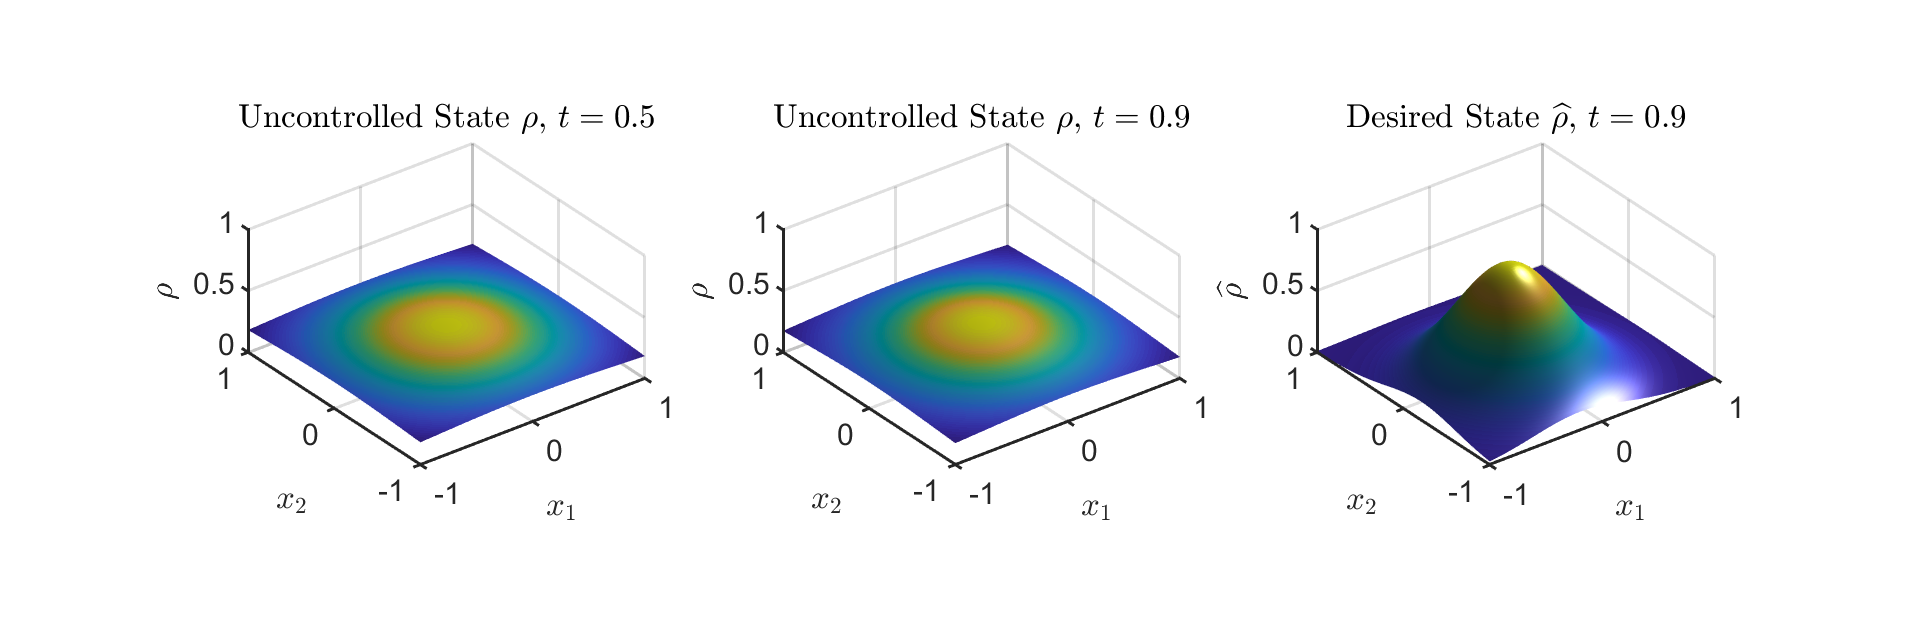
\includegraphics[scale=0.3]{Res1Ex4.png}
	\caption{2D Example 4, uncontrolled $\rho$ and $\widehat \rho$, $\beta = 10^{-3}$, $\gamma = -1$. ++Needs update++}
	\label{rhoHat2dEx4}
\end{figure}
\begin{figure}[h]
	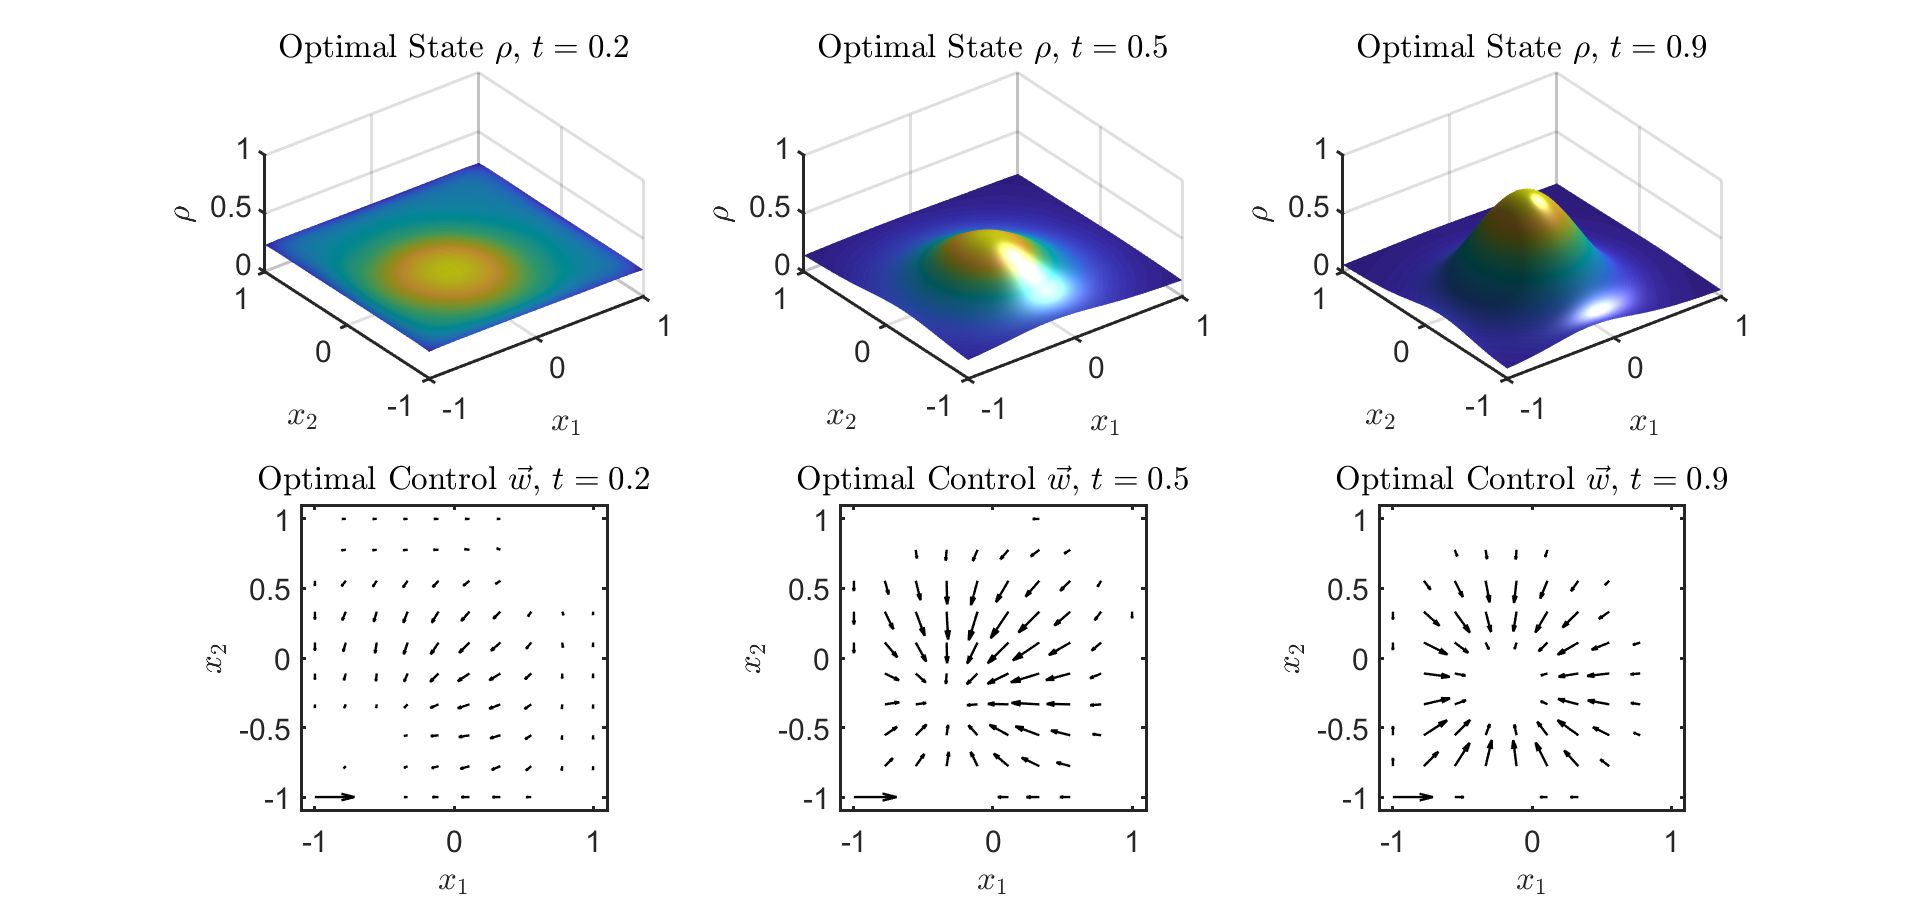
\includegraphics[scale=0.3]{Res2Ex4.png}
	\caption{2D Example 4, controlled $\rho$ and optimal control $\vec{w}$, $\beta = 10^{-3}$, $\gamma = -1$.++Needs update++}
	\label{rhoOpt2dEx4}
\end{figure}








